\documentclass[11pt,a4paper,oneside]{report}

% --- Кодировки и языки ---
\usepackage[utf8]{inputenc}
\usepackage[T2A]{fontenc}
\usepackage[russian]{babel}

% --- Математика и шрифты ---
\usepackage{amsmath,amssymb,amsthm,amsfonts}
\usepackage{mathtools}
\usepackage{microtype} 

% --- Геометрия страницы ---
\usepackage[left=1.0cm,right=1.0cm,top=1.5cm,bottom=1.5cm]{geometry}

% --- Графика ---
\usepackage{graphicx}

% --- Ссылки и цвета ---
\usepackage[dvipsnames]{xcolor}
\usepackage[colorlinks=true, linkcolor=blue, urlcolor=cyan]{hyperref}

% --- Рамки ---
\usepackage[most]{tcolorbox} 
\usepackage{fancyhdr}
\usepackage{datetime}

% --- Команда для билетов ---
\newcommand{\examquestion}[3]{
    \refstepcounter{section}
    \addcontentsline{toc}{section}{Вопрос #1. #2}
    \vspace{1.5em}
    \begin{tcolorbox}[
        enhanced, breakable, 
        colback=white, colframe=black, coltext=black,
        boxrule=0.5pt, arc=0pt, 
        borderline={0.5pt}{0pt}{black, dashed}
    ]
    {\Large\bfseries Вопрос #1. #2}\par\vspace{0.5em}
    {\small\itshape #3}
    \end{tcolorbox}
    \vspace{0.5em}
}

% --- Теоремы и прочее ---
\theoremstyle{definition}
\newtheorem{definition}{Определение}
\theoremstyle{plain}
\newtheorem{theorem}{Теорема}
\newtheorem{lemma}{Лемма}
\newtheorem{property}{Свойство}
\newtheorem{example}{Пример}

% --- Метаданные ---
\title{
    \centering
    \Huge\bfseries Конспект по математическому анализу \\[0.5em]
    \vspace{1em}
    {\footnotesize\normalfont v. \ifnum\day<10 0\fi\the\day/\ifnum\month<10 0\fi\the\month \ \currenttime} \\[0.5em] 
    \vspace{5em}
    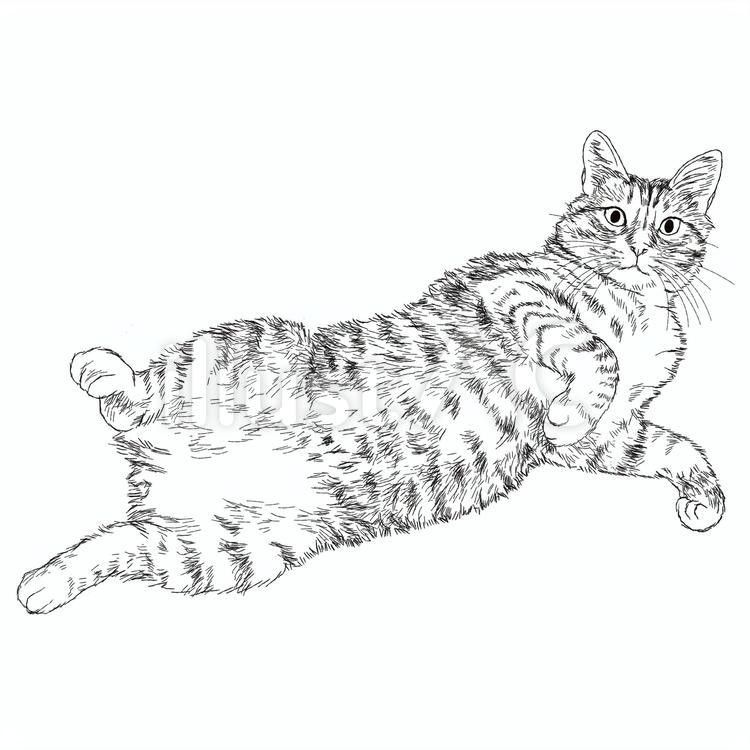
\includegraphics[width=0.5\textwidth]{cat.png} 
}
\author{}
\date{
    \vspace{\fill}
    {\scriptsize ITMO SE y29. Rzhonsnicskaya J.B. \& Gonchar L.I. course. \\[0.5em] "Every person with higher education must go through a BEE" \\[0.5em]}
}

\begin{document}

\maketitle 

\tableofcontents
\newpage

\clearpage
\section*{Пятёрка 1. Вопросы 1–5}

% --- Вопрос 1 ---
\examquestion{1}{Метод интегрирования по частям в неопределенном интеграле}
{Проведите вывод формулы интегрирования по частям, опираясь на дифференциал произведения двух функций. Перечислите и классифицируйте три основных типа интегралов, берущихся данным методом (с примерами шаблонов для каждого типа).}

\paragraph{Теоретическое обоснование и вывод формулы.}
Пусть на некотором промежутке заданы две функции $u(x)$ и $v(x)$, непрерывно дифференцируемые на этом промежутке. По правилу дифференцирования произведения, дифференциал функции $u(x)v(x)$ имеет вид:
$$ d(uv) = u \, dv + v \, du $$
В силу операции интегрирования, которая является обратной к дифференцированию, непрерывные функции в правой части равенства имеют первообразные. Интегрируя левую и правой части, в силу свойства линейности неопределенного интеграла получаем:
$$ \int d(uv) = \int (u \, dv + v \, du) = \int u \, dv + \int v \, du $$
По свойству неопределенного интеграла от дифференциала функции, левая часть равна $uv$ (с точностью до константы). Таким образом:
$$ uv = \int u \, dv + \int v \, du $$
Выражая интеграл $\int u \, dv$, получаем классическую формулу интегрирования по частям:
$$ \int u \, dv = uv - \int v \, du $$
Смысл данной формулы заключается в том, что вычисление интеграла $\int u \, dv$ сводится к вычислению другого интеграла $\int v \, du$, который при правильном выборе функций $u$ и $v$ оказывается существенно проще исходного.

\paragraph{Классификация трех основных типов интегралов:}
\begin{enumerate}
    \item \textbf{Тип I (Понижение степени многочлена):} Интегралы вида $\int P_n(x) e^{ax} dx$, $\int P_n(x) \sin(bx) dx$, $\int P_n(x) \cos(bx) dx$, где $P_n(x)$ — многочлен степени $n$. В данном случае за $u$ целесообразно выбирать многочлен $u = P_n(x)$, так как при его дифференцировании степень уменьшается ($du = P_n'(x)dx$), а в качестве $dv$ берется оставшаяся тригонометрическая или показательная часть, легко интегрируемая методом табличных значений. Шаг повторяется $n$ раз до полного исчезновения многочлена.
    
    \item \textbf{Тип II (Переход к алгебраическим дробям):} Интегралы вида $\int P_n(x) \ln x \, dx$, $\int P_n(x) \arcsin x \, dx$, $\int P_n(x) \arctan x \, dx$. Здесь за $u$ выбирается трансцендентная функция ($u = \ln x$ или $u = \arctan x$), поскольку операция дифференцирования превращает её в алгебраическое выражение. В качестве $dv$ берется многочлен с дифференциалом $dv = P_n(x)dx$, интегрирование которого дает функцию $v$, являющуюся многочленом степени $n+1$. После применения формулы интегрирования по частям новый интеграл представляет собой интегрирование рациональной дроби.
    
    \item \textbf{Тип III (Циклические интегралы):} Интегралы вида $\int e^{ax} \sin(bx) dx$ и $\int e^{ax} \cos(bx) dx$. Особенность данного типа заключается в том, что ни показательная, ни тригонометрическая функции не упрощаются при дифференцировании или интегрировании. Применяя формулу по частям дважды (выбирая на каждом шаге за $u$ функции одного класса — либо всегда экспоненту, либо всегда тригонометрию), мы возвращаемся к исходному интегралу, формируя линейное уравнение относительно искомого интеграла.
\end{enumerate}

\paragraph{Бонус-пример на каждый тип:}
\begin{itemize}
    \item \textbf{Пример для Типа I:} Вычислим интеграл $\int x e^{2x} dx$. Пусть $u = x \implies du = dx$, а $dv = e^{2x} dx \implies v = \frac{1}{2}e^{2x}$. Тогда:
    $$ \int x e^{2x} dx = x \cdot \left(\frac{1}{2}e^{2x}\right) - \int \frac{1}{2}e^{2x} dx = \frac{x}{2}e^{2x} - \frac{1}{4}e^{2x} + C = \frac{e^{2x}}{4}(2x - 1) + C. $$
    
    \item \textbf{Пример для Типа II:} Вычислим интеграл $\int \ln x \, dx$. Пусть $u = \ln x \implies du = \frac{1}{x}dx$, а $dv = dx \implies v = x$. Применяем формулу:
    $$ \int \ln x \, dx = x \ln x - \int x \cdot \frac{1}{x} dx = x \ln x - \int dx = x \ln x - x + C. $$
    
    \item \textbf{Пример для Типа III:} Найдем интеграл $I = \int e^x \cos x \, dx$. Пусть $u = e^x \implies du = e^x dx$, а $dv = \cos x \, dx \implies v = \sin x$. Получаем:
    $$ I = e^x \sin x - \int e^x \sin x \, dx $$
    Применим метод по частям к полученному интегралу повторно, удерживая выбор $u$ за экспонентой: $u = e^x \implies du = e^x dx$, $dv = \sin x \, dx \implies v = -\cos x$.
    $$ I = e^x \sin x - \left( -e^x \cos x - \int (-\cos x) e^x dx \right) = e^x \sin x + e^x \cos x - \int e^x \cos x \, dx $$
    Замечаем, что последний интеграл равен $I$. Получаем алгебраическое уравнение:
    $$ I = e^x(\sin x + \cos x) - I \implies 2I = e^x(\sin x + \cos x) \implies I = \frac{e^x(\sin x + \cos x)}{2} + C. $$
\end{itemize}







% --- Вопрос 2 ---
\examquestion{2}{Метод замены переменной (подстановки) в неопределенном интеграле}
{Сформулируйте и докажите теорему о замене переменной. Покажите на конкретном примере, как этот метод применяется для раскрытия циклических тригонометрических интегралов.}

\begin{theorem}[О замене переменной]
Пусть функция $x = \varphi(t)$ определена и дифференцируема на промежутке $T$, а её множество значений представляет собой промежуток $X$. Пусть функция $f(x)$ определена на промежутке $X$ и имеет на нем первообразную $F(x)$, то есть $F'(x) = f(x)$. Тогда на промежутке $T$ функция $f(\varphi(t))\varphi'(t)$ имеет первообразную $F(\varphi(t))$, и справедлива формула:
$$ \int f(\varphi(t)) \varphi'(t) dt = \left. \int f(x) dx \right|_{x = \varphi(t)} = F(\varphi(t)) + C $$
\end{theorem}

\begin{proof}
Для доказательства данного тождества достаточно показать, что функция $F(\varphi(t))$ является первообразной для подынтегральной функции в левой части равенства. Согласно определению, продифференцируем сложную функцию $F(\varphi(t))$ по переменной $t$, используя правило дифференцирования сложной функции:
$$ \frac{d}{dt} \Big( F(\varphi(t)) \Big) = F'(\varphi(t)) \cdot \varphi'(t) $$
Так как по условию теоремы $F'(x) = f(x)$, то, подставляя аргумент $x = \varphi(t)$, имеем $F'(\varphi(t)) = f(\varphi(t))$. Отсюда получаем:
$$ \frac{d}{dt} \Big( F(\varphi(t)) \Big) = f(\varphi(t)) \varphi'(t) $$
Поскольку производная функции $F(\varphi(t))$ по переменной $t$ в точности совпадает с подынтегральной функцией, то по определению неопределенного интеграла множество всех первообразных имеет вид $F(\varphi(t)) + C$, что завершает доказательство теоремы.
\end{proof}

\paragraph{Пример (Раскрытие циклического тригонометрического интеграла).}
Рассмотрим интеграл от нечетной степени тригонометрической функции, порождающий циклический переход при неверном подходе, но эффективно раскрываемый подстановкой: $I = \int \sin^3 x \cos^2 x \, dx$.
Используем основное тригонометрическое тождество, чтобы выделить один дифференциал синуса: $\sin^3 x = \sin^2 x \cdot \sin x = (1 - \cos^2 x)\sin x$. Тогда:
$$ I = \int (1 - \cos^2 x)\cos^2 x \cdot \sin x \, dx $$
Сделаем замену переменной $t = \cos x$. Находим дифференциал: $dt = -\sin x \, dx \implies \sin x \, dx = -dt$. Пересчитаем интеграл относительно переменной $t$:
$$ I = \int (1 - t^2)t^2 (-dt) = \int (t^4 - t^2) dt = \frac{t^5}{5} - \frac{t^3}{3} + C $$
Возвращаясь к исходной переменной $x$, получаем окончательный ответ:
$$ I = \frac{\cos^5 x}{5} - \frac{\cos^3 x}{3} + C. $$

\paragraph{Бонус-пример (Универсальная тригонометрическая подстановка):}
Вычислим $I = \int \frac{dx}{2 + \cos x}$. Сделаем стандартную подстановку $t = \tan \frac{x}{2}$. Тогда выразим $dx = \frac{2dt}{1+t^2}$ и $\cos x = \frac{1-t^2}{1+t^2}$. Подставляем в интеграл:
$$ I = \int \frac{\frac{2dt}{1+t^2}}{2 + \frac{1-t^2}{1+t^2}} = \int \frac{2dt}{2(1+t^2) + (1-t^2)} = \int \frac{2dt}{3 + t^2} = \frac{2}{\sqrt{3}} \arctan\left(\frac{t}{\sqrt{3}}\right) + C $$
Выполняя обратную замену, находим: $I = \frac{2}{\sqrt{3}} \arctan\left(\frac{\tan(x/2)}{\sqrt{3}}\right) + C$.





% --- Вопрос 3 ---
\examquestion{3}{Complex method v veschestvennom analize}
{Опираясь на свойства комплексной экспоненты и формулу Эйлера, проведите вывод формул для интегралов вида $I_{1}=\int e^{ax}\cos(bx)dx$ и $I_{2}=\int e^{ax}\sin(bx)dx$, где $a,b\in\mathbb{R}$. Докажите корректность перехода к комплексному интегралу $\int e^{(a+ib)x}dx$ и последующего разделения вещественной и мнимой частей.}

\paragraph{Суть метода и итоговые формулы.}
При классическом подходе интегралы вида $I_1 = \int e^{ax}\cos(bx)dx$ и $I_2 = \int e^{ax}\sin(bx)dx$ вычисляются двукратным интегрированием по частям, что приводит к громоздким циклическим уравнениям. 

Комплексный метод позволяет найти оба интеграла одновременно и чисто алгебраическим путём. Для этого вводится вспомогательный комплексный интеграл $J = \int e^{(a+ib)x} dx$. Согласно формуле Эйлера, его вещественная часть ($\text{Re}\,J$) в точности равна интегралу $I_1$, а мнимая часть ($\text{Im}\,J$) — интегралу $I_2$.

В результате интегрирования комплексной экспоненты получаются следующие **итоговые формулы**:
$$ \int e^{ax}\cos(bx)dx = \frac{e^{ax}(a\cos bx + b\sin bx)}{a^2+b^2} + C $$
$$ \int e^{ax}\sin(bx)dx = \frac{e^{ax}(a\sin bx - b\cos bx)}{a^2+b^2} + C $$
Ниже приведено строгое обоснование этого перехода и пошаговый алгебраический вывод.

\paragraph{Доказательство корректности перехода.}
Пусть задана комплексная функция вещественного аргумента $w(x) = u(x) + i v(x)$, где $u(x), v(x)$ — вещественные функции, непрерывные на рассматриваемом промежутке. По определению, интеграл от такой функции равен:
$$ \int w(x) dx = \int (u(x) + i v(x)) dx = \int u(x) dx + i \int v(x) dx $$
Формула Эйлера задает связь комплексной экспоненты с тригонометрическими функциями: $e^{i\varphi} = \cos\varphi + i\sin\varphi$. Применим её к функции $e^{(a+ib)x}$:
$$ e^{(a+ib)x} = e^{ax} \cdot e^{ibx} = e^{ax}(\cos(bx) + i \sin(bx)) = e^{ax}\cos(bx) + i e^{ax}\sin(bx) $$
Интегрируя это выражение по определению, получаем:
$$ \int e^{(a+ib)x} dx = \int e^{ax}\cos(bx) dx + i \int e^{ax}\sin(bx) dx = I_1 + i I_2 $$
Поскольку операция выделения вещественной ($\text{Re}$) и мнимой ($\text{Im}$) частей коммутирует с интегрированием, мы можем утверждать:
$$ I_1 = \text{Re} \left( \int e^{(a+ib)x} dx \right), \quad I_2 = \text{Im} \left( \int e^{(a+ib)x} dx \right) $$
Так как закон дифференцирования $\frac{d}{dx} e^{kx} = k e^{kx}$ выполняется на комплексной плоскости для любого $k = a+ib \in \mathbb{C}$, операция вычисления первообразной от комплексной экспоненты полностью эквивалентна вещественному аналогу: $\int e^{kx} dx = \frac{1}{k} e^{kx} + C$.

\paragraph{Вывод формул.}
Вычислим комплексный интеграл в явном виде:
$$ \int e^{(a+ib)x} dx = \frac{e^{(a+ib)x}}{a+ib} = \frac{e^{ax}(\cos bx + i \sin bx)}{a+ib} $$
Для разделения вещественной и мнимой частей избавимся от комплексности в знаменателе, умножив числитель и знаменатель на сопряженное число $(a-ib)$:
$$ \frac{e^{ax}(\cos bx + i \sin bx)(a-ib)}{(a+ib)(a-ib)} = \frac{e^{ax}}{a^2+b^2} \Big( a\cos bx - i b\cos bx + i a\sin bx - i^2 b\sin bx \Big) $$
Учитывая, что $i^2 = -1$, сгруппируем слагаемые на вещественные и мнимые компоненты:
$$ \int e^{(a+ib)x} dx = \frac{e^{ax}}{a^2+b^2} \Big( (a\cos bx + b\sin bx) + i(a\sin bx - b\cos bx) \Big) $$
Выделяя вещественную и мнимую части, получаем искомые формулы для интегралов:
$$ I_1 = \int e^{ax}\cos(bx)dx = \frac{e^{ax}(a\cos bx + b\sin bx)}{a^2+b^2} + C $$
$$ I_2 = \int e^{ax}\sin(bx)dx = \frac{e^{ax}(a\sin bx - b\cos bx)}{a^2+b^2} + C $$

\paragraph{Бонус-пример:} Вычислим интеграл $\int e^{3x} \sin(2x) dx$. 
В данном случае параметры $a = 3$, $b = 2$. Прямым подстановлением в выведенную формулу для $I_2$ получаем:
$$ \int e^{3x} \sin(2x) dx = \frac{e^{3x}(3\sin 2x - 2\cos 2x)}{3^2+2^2} + C = \frac{e^{3x}(3\sin 2x - 2\cos 2x)}{13} + C. $$








% --- Вопрос 4 ---
\examquestion{4}{Методы нахождения неопределенных коэффициентов}
{Проведите сравнительный анализ метода приравнивания коэффициентов при одинаковых степенях и метода частных значений. Дайте обоснование методу вычетов Хевисайда для случая простых линейных множителей в знаменателе.}

\paragraph{Правила формирования структуры числителей элементарных дробей.}
При разложении правильной рациональной дроби $\frac{P(x)}{Q(x)}$ вид многочлена в числителе каждой элементарной дроби однозначно определяется структурой сомножителей в знаменателе:
\begin{itemize}
    \item \textbf{Принцип формирования:} Степень многочлена в числителе должна быть строго на единицу меньше степени базового многочлена, находящегося внутри скобки знаменателя (без учета внешней кратности этой скобки).
    \item \textbf{Линейный сомножитель} $(x - a)^k$: Внутреннее выражение $x - a$ является многочленом первой степени ($x^1$). Следовательно, в числителе формируется многочлен нулевой степени — константа ($A$). Количество дробей в группе равно кратности $k$:
    $$ \frac{A_1}{x-a} + \frac{A_2}{(x-a)^2} + \dots + \frac{A_k}{(x-a)^k} $$
    \item \textbf{Квадратичный сомножитель} $(x^2 + px + q)^m$ с отрицательным дискриминантом ($D < 0$): Внутреннее выражение является многочленом второй степени ($x^2$). Следовательно, в числителе формируется линейный двухчлен — многочлен первой степени ($Bx + C$). Количество дробей равно кратности $m$:
    $$ \frac{B_1 x + C_1}{x^2 + px + q} + \frac{B_2 x + C_2}{(x^2 + px + q)^2} + \dots + \frac{B_m x + C_m}{(x^2 + px + q)^m} $$
\end{itemize}

\paragraph{Теоретическое обоснование разложения.}
Любая правильная рациональная дробь $\frac{P(x)}{Q(x)}$ над полем действительных чисел допускает единственное разложение на сумму элементарных дробей указанных типов. 
\begin{itemize}
    \item Каждому действительному корню $x = a$ кратности $k$ соответствует группа из $k$ дробей вида: $\sum_{i=1}^{k} \frac{A_i}{(x-a)^i}$, где $A_i \in \mathbb{R}$.
    \item Каждой паре комплексно-сопряженных корней кратности $m$ соответствует группа из $m$ дробей вида: $\sum_{j=1}^{m} \frac{B_j x + C_j}{(x^2+px+q)^j}$, где $B_j, C_j \in \mathbb{R}$.
\end{itemize}

\paragraph{Сравнительный анализ методов определения коэффициентов.}
После приведения всех элементарных дробей к общему знаменателю $Q(x)$ фиксируется тождественное равенство исходного числителя $P(x)$ и полученного многочлена с неопределенными коэффициентами $M(x)$: $P(x) \equiv M(x)$. Для нахождения неизвестных применяются два метода:

\begin{enumerate}
    \item \textbf{Метод частных значений:}
    \\ Основан на свойстве тождественности: равенство справедливо при любых значениях переменной $x$. В уравнение подставляются действительные корни знаменателя $Q(x)$, что приводит к занулению большинства слагаемых и мгновенному нахождению части коэффициентов.
    \\ \textit{Преимущества:} Высокая скорость вычислений. При наличии только простых действительных корней исключает необходимость решения систем уравнений.
    \\ \textit{Недостатки:} При наличии комплексных или кратных корней метод не позволяет напрямую определить все неизвестные. Требуется подстановка искусственных значений (например, $x=0$, $x=1$) и комбинирование с другими подходами.
    
    \item \textbf{Метод приравнивания коэффициентов:}
    \\ Основан на теореме о равенстве многочленов: два многочлена тождественно равны тогда и только тогда, когда равны их коэффициенты при одинаковых степенях переменной $x^k$. Проводится полное раскрытие скобок в $M(x)$, группировка по степеням $x$ и составление системы линейных алгебраических уравнений (СЛАУ).
    \\ \textit{Преимущества:} Абсолютная универсальность. Метод применим для любых типов и кратностей корней знаменателя.
    \\ \textit{Недостатки:} Высокая вычислительная трудоемкость. При больших степенях знаменателя приводит к громоздким СЛАУ, требующим применения метода Гаусса.
\end{enumerate}

\paragraph{Обоснование метода вычетов Хевисайда.}
Пусть рациональная дробь имеет вид $\frac{P(x)}{Q(x)}$, где знаменатель содержит простой линейный корень $x = x_1$ кратности $1$. Тогда многочлен знаменателя представим в виде $Q(x) = (x - x_1)R(x)$, причем $R(x_1) \neq 0$. 

Выделим из общего разложения дробь с искомым коэффициентом $A_1$:
$$ \frac{P(x)}{(x-x_1)R(x)} = \frac{A_1}{x-x_1} + \sum \text{оставшиеся дроби} $$
Умножим обе части тождества на линейный множитель $(x - x_1)$:
$$ \frac{P(x)}{R(x)} = A_1 + (x - x_1) \cdot \sum \text{оставшиеся дроби} $$
Перейдем к пределу при $x \to x_1$. Поскольку сумма оставшихся дробей представляет собой правильную рациональную функцию, не имеющую особенностей в точке $x_1$, произведение второго слагаемого на $(x-x_1)$ стремится к нулю. Получаем явное выражение для коэффициента:
$$ A_1 = \lim_{x \to x_1} \frac{P(x)}{R(x)} = \frac{P(x_1)}{R(x_1)} $$
Применим правило дифференцирования произведения к знаменателю: $Q'(x) = R(x) + (x - x_1)R'(x)$. При подстановке значения $x = x_1$ второе слагаемое обращается в нуль: $Q'(x_1) = R(x_1)$. Таким образом, получаем классическую предельную формулу Хевисайда:
$$ A_1 = \frac{P(x_1)}{Q'(x_1)} $$

\paragraph{Пример практического применения (Метод Хевисайда):}
Разложим правильную дробь $\frac{2x + 3}{(x-2)(x+3)} = \frac{A}{x-2} + \frac{B}{x+3}$.
\begin{itemize}
    \item Нахождение коэффициента $A$ при корне $x = 2$ путем исключения сомножителя $(x-2)$ из исходного знаменателя:
    $$ A = \left. \frac{2x + 3}{x + 3} \right|_{x=2} = \frac{2(2) + 3}{2 + 3} = \frac{7}{5} $$
    \item Нахождение коэффициента $B$ при корне $x = -3$ путем исключения сомножителя $(x+3)$ из исходного знаменателя:
    $$ B = \left. \frac{2x + 3}{x - 2} \right|_{x=-3} = \frac{2(-3) + 3}{-3 - 2} = \frac{-3}{-5} = \frac{3}{5} $$
\end{itemize}
Результат разложения: $\frac{2x + 3}{(x-2)(x+3)} = \frac{7}{5(x-2)} + \frac{3}{5(x+3)}$.

% --- Вопрос 5 ---
\examquestion{5}{Интегрирование элементарных дробей IV типа}
{Выведите рекуррентную формулу для вычисления интеграла от элементарной дроби IV типа: $I_{n}=\int\frac{dx}{(x^{2}+a^{2})^{n}}$, $n\in\mathbb{N}$. Покажите этап интегрирования по частям и алгоритм понижения степени знаменателя.}

\paragraph{План вывода кратко:}
\begin{enumerate}
    \item \textbf{Подмена в числителе:} $1 = \frac{1}{a^2} \cdot \frac{(x^2+a^2) - x^2}{(x^2+a^2)^n} \implies$ разбиваем на $I_{n-1}$ и «хвост» с $x^2$.
    \item \textbf{Части для «хвоста»:} Интеграл $\int \frac{x \cdot x \, dx}{(x^2+a^2)^n}$ берем по частям:
    \begin{itemize}
        \item $u = x \implies du = dx$
        \item $dv = \frac{x \, dx}{(x^2+a^2)^n} \implies v = \frac{(x^2+a^2)^{-n+1}}{2(1-n)}$
    \end{itemize}
    \item \textbf{Сборка:} Подставляем всё в уравнение $I_n = \frac{1}{a^2}I_{n-1} - \frac{1}{a^2}I^*$ и приводим подобные при $I_{n-1}$.
\end{enumerate}

\begin{tcolorbox}[colback=white, colframe=black, boxrule=0.5pt, arc=0pt, borderline={0.5pt}{0pt}{black, dashed}]
    \centering
    $$ I_n = \frac{x}{2a^2(n-1)(x^2+a^2)^{n-1}} + \frac{2n-3}{2a^2(n-1)} I_{n-1} $$
\end{tcolorbox}
\paragraph{Математический вывод формулы.}
Рассмотрим интеграл элементарной дроби IV типа: $I_n = \int \frac{dx}{(x^2+a^2)^n}$. Реализуем первый этап алгоритма:
$$ I_n = \frac{1}{a^2} \int \frac{a^2}{(x^2+a^2)^n} dx = \frac{1}{a^2} \int \frac{(x^2+a^2) - x^2}{(x^2+a^2)^n} dx $$
Используя свойство линейности неопределенного интеграла, разобьем выражение на два отдельных слагаемых:
$$ I_n = \frac{1}{a^2} \int \frac{x^2+a^2}{(x^2+a^2)^n} dx - \frac{1}{a^2} \int \frac{x^2}{(x^2+a^2)^n} dx $$
После сокращения первой дроби получаем соотношение, связывающее $I_n$ и $I_{n-1}$:
$$ I_n = \frac{1}{a^2} I_{n-1} - \frac{1}{a^2} I^*, \quad \text{где } I^* = \int \frac{x \cdot x \, dx}{(x^2+a^2)^n} $$
Перейдем ко второму этапу — интегрированию по частям интеграла $I^*$. Пусть:
$$ u = x \implies du = dx $$
$$ dv = \frac{x \, dx}{(x^2+a^2)^n} = \frac{1}{2} (x^2+a^2)^{-n} d(x^2+a^2) \implies v = \frac{1}{2(1-n)(x^2+a^2)^{n-1}} $$
Применяя классическую формулу $\int u \, dv = uv - \int v \, du$, преобразуем интеграл $I^*$:
$$ I^* = \frac{x}{2(1-n)(x^2+a^2)^{n-1}} - \int \frac{dx}{2(1-n)(x^2+a^2)^{n-1}} $$
Вынесем константу за знак интеграла, сводя его к определению $I_{n-1}$:
$$ I^* = \frac{x}{2(1-n)(x^2+a^2)^{n-1}} - \frac{1}{2(1-n)} I_{n-1} $$
Перейдем к третьему этапу. Подставим полученное выражение для $I^*$ в исходное уравнение для $I_n$:
$$ I_n = \frac{1}{a^2} I_{n-1} - \frac{1}{a^2} \left[ \frac{x}{2(1-n)(x^2+a^2)^{n-1}} - \frac{1}{2(1-n)} I_{n-1} \right] $$
Для упрощения знаков преобразуем константу в знаменателе: $\frac{1}{2(1-n)} = -\frac{1}{2(n-1)}$. Раскроем скобки:
$$ I_n = \frac{x}{2a^2(n-1)(x^2+a^2)^{n-1}} + \frac{1}{a^2} I_{n-1} - \frac{1}{2a^2(n-1)} I_{n-1} $$
Сгруппируем слагаемые при интеграле $I_{n-1}$, приведя их коэффициенты к общему знаменателю $2a^2(n-1)$:
$$ \frac{1}{a^2} - \frac{1}{2a^2(n-1)} = \frac{2(n-1) - 1}{2a^2(n-1)} = \frac{2n - 3}{2a^2(n-1)} $$
В результате получаем окончательную рекуррентную формулу понижения степени для интегралов IV типа:
$$ I_n = \frac{x}{2a^2(n-1)(x^2+a^2)^{n-1}} + \frac{2n-3}{2a^2(n-1)} I_{n-1} $$

\paragraph{Пример практического применения:} Вычислим интеграл $I_2 = \int \frac{dx}{(x^2+4)^2}$.
В данном случае параметры имеют значения $a^2 = 4 \implies a = 2$, начальная степень $n = 2$. 
Базовый табличный интеграл первого порядка ($n=1$) равен:
$$ I_1 = \int \frac{dx}{x^2+4} = \frac{1}{2} \arctan\left(\frac{x}{2}\right) $$
Подставим параметры $n=2$ и $a^2=4$ в выведенную рекуррентную формулу:
$$ I_2 = \frac{x}{2 \cdot 4 \cdot (2-1)(x^2+4)^{2-1}} + \frac{2(2)-3}{2 \cdot 4 \cdot (2-1)} I_1 = \frac{x}{8(x^2+4)} + \frac{1}{8} I_1 $$
Подставляя явный вид интеграла $I_1$ и добавляя константу интегрирования, получаем финальный результат:
$$ I_2 = \frac{x}{8(x^2+4)} + \frac{1}{16} \arctan\left(\frac{x}{2}\right) + C $$
\clearpage
\section*{Пятёрка 2. Вопросы 6–10}

% --- Вопрос 6 ---
\examquestion{6}{Метод Остроградского}
{Дайте обоснование методу выделения рациональной части интеграла от правильной рациональной дроби, знаменатель которой имеет кратные корни. Докажите корректность дифференцирования основного уравнения Остроградского для перехода к алгебраической системе линейных уравнений.}

\paragraph{Теоретическое обоснование метода.}
Пусть задан интеграл от правильной рациональной дроби $\int \frac{P(x)}{Q(x)} dx$, где многочлен знаменателя $Q(x)$ имеет кратные корни (действительные или комплексные), то есть его каноническое разложение имеет вид $Q(x) = (x-x_1)^{k_1}\dots(x^2+p_1x+q_1)^{m_1}\dots$. Традиционное разложение такой дроби на элементарные приводит к дробям высоких порядков, интегрирование которых требует применения громоздких рекуррентных формул понижения степени знаменателя.

Метод Остроградского позволяет обойти эту процедуру и чисто алгебраически выделить рациональную (алгебраическую) часть интеграла от трансцендентной части (логарифмы, арктангенсы). Основное уравнение метода имеет вид:
$$ \int \frac{P(x)}{Q(x)} dx = \frac{X(x)}{Q_1(x)} + \int \frac{Y(x)}{Q_2(x)} dx $$
где структура новых знаменателей однозначно определяется по исходному знаменателю $Q(x)$:
\begin{enumerate}
    \item $Q_1(x) = \text{НОД}(Q(x), Q'(x))$ — многочлен, содержащий все те же корни, что и $Q(x)$, но их кратности снижены ровно на единицу. Таким образом, $\frac{X(x)}{Q_1(x)}$ является искомой рациональной частью первообразной.
    \item $Q_2(x) = \frac{Q(x)}{Q_1(x)}$ — многочлен, содержащий все корни знаменателя $Q(x)$, но строго первой кратности. Дробь $\frac{Y(x)}{Q_2(x)}$ под интегралом даст исключительно трансцендентные функции.
\end{enumerate}
Степени неопределенных многочленов числителей выбираются на единицу меньше степеней соответствующих знаменателей: $\deg X = \deg Q_1 - 1$, $\deg Y = \deg Q_2 - 1$.

\paragraph{Доказательство корректности дифференцирования.}
Для нахождения коэффициентов многочленов $X(x)$ и $Y(x)$ выполним операцию дифференцирования обеих частей основного уравнения по переменной $x$. На основании основной теоремы дифференциального исчисления, производная от неопределенного интеграла по его верхнему пределу равна подынтегральной функции:
$$ \frac{P(x)}{Q(x)} = \frac{X'(x)Q_1(x) - X(x)Q_1'(x)}{Q_1^2(x)} + \frac{Y(x)}{Q_2(x)} $$
Докажем, что полученное уравнение легко сводится к линейной системе уравнений. Умножим обе части равенства на исходный многочлен $Q(x)$. Учитывая, что по определению $Q(x) = Q_1(x)Q_2(x)$, получаем:
$$ P(x) = \frac{\big(X'(x)Q_1(x) - X(x)Q_1'(x)\big) \cdot Q_1(x)Q_2(x)}{Q_1^2(x)} + \frac{Y(x) \cdot Q_1(x)Q_2(x)}{Q_2(x)} $$
Сокращая дроби, приходим к уравнению:
$$ P(x) = \frac{X'(x)Q_1(x)Q_2(x) - X(x)Q_1'(x)Q_2(x)}{Q_1(x)} + Y(x)Q_1(x) $$
Поскольку $Q_2(x) = \frac{Q(x)}{Q_1(x)}$, то выражение $\frac{Q_1'(x)Q_2(x)}{Q_1(x)}$ является целым многочленом. Действительно, $Q'(x) = (Q_1(x)Q_2(x))' = Q_1'(x)Q_2(x) + Q_1(x)Q_2'(x)$. Разделив на $Q_1(x)$, видим, что все слагаемые целочисленны по структуре степеней. Окончательно получаем алгебраическое тождество многочленов:
$$ P(x) = X'(x)Q_2(x) - X(x) \, \frac{Q_1'(x)Q_2(x) - Q'(x)}{Q_1(x)} + Y(x)Q_1(x) $$
Левая и правая части полученного тождества представляют собой многочлены. Приравнивая коэффициенты при одинаковых степенях $x$, мы получаем совместную систему линейных алгебраических уравнений. Корректность гарантируется линейной независимостью базисных дробей разложения.

\paragraph{Бонус-пример:} Применим метод к интегралу $\int \frac{dx}{(x^2-1)^2}$. Здесь $Q(x) = (x^2-1)^2$.
\begin{itemize}
    \item Находим знаменатели: $Q'(x) = 2(x^2-1)\cdot 2x = 4x(x^2-1)$. Тогда $Q_1(x) = \text{НОД}(Q, Q') = x^2-1$. Соответственно, $Q_2(x) = \frac{Q(x)}{Q_1(x)} = x^2-1$.
    \item Записываем структуру числителей: так как $\deg Q_1 = 2$ и $\deg Q_2 = 2$, то $\deg X = 1 \implies X(x) = Ax + B$, $\deg Y = 1 \implies Y(x) = Cx + D$.
    \item Формула Остроградского: $\int \frac{dx}{(x^2-1)^2} = \frac{Ax+B}{x^2-1} + \int \frac{Cx+D}{x^2-1} dx$. Дифференцируем:
    $$ \frac{1}{(x^2-1)^2} = \frac{A(x^2-1) - 2x(Ax+B)}{(x^2-1)^2} + \frac{Cx+D}{x^2-1} \implies 1 = A(x^2-1) - 2x(Ax+B) + (Cx+D)(x^2-1) $$
    Раскрывая скобки и приравнивая коэффициенты, находим: $A = 0, B = -1/2, C = 0, D = -1/2$.
    \item Итог: $\int \frac{dx}{(x^2-1)^2} = -\frac{x}{2(x^2-1)} - \frac{1}{4}\ln\left|\frac{x-1}{x+1}\right| + C$.
\end{itemize}

% --- Вопрос 7 ---
\examquestion{7}{Интегрирование дробно-линейных иррациональностей}
{Опираясь на понятие рационализирующей подстановки, подробно разберите метод интегрирования выражений, содержащих дробно-линейные иррациональности вида $\sqrt[n]{\frac{ax+b}{cx+d}}$. Докажите теорему о сведении таких интегралов к интегралам от рациональных функций.}

\begin{theorem}[О рационализации дробно-линейных иррациональностей]
Интеграл вида $\int R\left(x, \sqrt[n]{\frac{ax+b}{cx+d}}\right) dx$, где $R$ — рациональная функция своих аргументов, а $ad - bc \neq 0$, с помощью подстановки $t = \sqrt[n]{\frac{ax+b}{cx+d}}$ всегда сводится к интегралу от рациональной функции переменной $t$.
\end{theorem}

\begin{proof}
Пусть $t = \sqrt[n]{\frac{ax+b}{cx+d}}$. Для доказательства теоремы необходимо показать, что переменная $x$ и её дифференциал $dx$ выражаются через целые рациональные степени переменной $t$. Возведем обе части равенства в степень $n$:
$$ t^n = \frac{ax+b}{cx+d} $$
Выразим отсюда $x$. Для этого умножим обе части на знаменатель $cx+d$:
$$ t^n(cx + d) = ax + b \implies c x t^n + d t^n = a x + b \implies x(c t^n - a) = b - d t^n $$
Отсюда получаем явное выражение для переменной $x$ как рациональной функции от $t$:
$$ x = \frac{b - d t^n}{c t^n - a} = \psi(t) $$
Поскольку функция $\psi(t)$ является дробно-рациональной (отношение двух многочленов), её производная по переменной $t$ также будет являться дробно-рациональной функцией. Найдем дифференциал $dx$:
$$ dx = \psi'(t)dt = \frac{(-d \cdot n t^{n-1})(c t^n - a) - (b - d t^n)(c \cdot n t^{n-1})}{(c t^n - a)^2} dt = \frac{n t^{n-1}(ad - bc)}{(c t^n - a)^2} dt $$
Подставим полученные выражения в исходный интеграл:
$$ \int R\left(x, \sqrt[n]{\frac{ax+b}{cx+d}}\right) dx = \int R\left( \psi(t), t \right) \psi'(t) dt $$
Так как суперпозиция и произведение рациональных функций представляют собой рациональную функцию, подынтегральное выражение становится чистой рациональной дробью от переменной $t$. Теорема доказана.
\end{proof}

\paragraph{Бонус-пример:} Вычислим интеграл $\int \frac{dx}{(1+x)\sqrt{x}}$.
Данный интеграл содержит простую линейную иррациональность $\sqrt{x}$. Сделаем замену $t = \sqrt{x} \implies x = t^2$, следовательно, $dx = 2t\,dt$. Подставляем выражения в исходный интеграл:
$$ \int \frac{2t\,dt}{(1+t^2) \cdot t} = 2 \int \frac{dt}{1+t^2} = 2 \arctan t + C $$
Выполняя обратную замену $t = \sqrt{x}$, получаем окончательный ответ: $2 \arctan\sqrt{x} + C$.

% --- Вопрос 8 ---
\examquestion{8}{Подстановки Эйлера}
{Сформулируйте геометрические и алгебраические предпосылки трех подстановок Эйлера для интегралов вида $\int R(x, \sqrt{ax^2+bx+c})dx$. Выведите формулы для первой и второй подстановок Эйлера, доказав их рационализирующий характер.}

\paragraph{Алгебраические предпосылки.}
Интегралы вида $\int R(x, \sqrt{ax^2+bx+c})dx$ не могут быть вычислены в элементарных функциях напрямую, если квадратный трехчлен не является полным квадратом. Эйлер предложил три подстановки, основанные на алгебраической структуре коэффициентов трехчлена, которые переводят кривую второго порядка в параметрический вид, выражаемый рациональными функциями.

\paragraph{Вывод первой подстановки Эйлера ($a > 0$).}
Если старший коэффициент квадратного трехчлена положителен, то при очень больших $x$ поведение корня близко к поведению функции $\pm \sqrt{a}x$. Это позволяет сделать замену:
$$ \sqrt{ax^2+bx+c} = \pm\sqrt{a}x + t $$
Выберем знак «+» и возведем обе части равенства в квадрат для уничтожения радикалов:
$$ ax^2 + bx + c = (\sqrt{a}x + t)^2 = ax^2 + 2\sqrt{a}xt + t^2 $$
Слагаемые $ax^2$ в левой и правой частях взаимно уничтожаются, что линеаризует уравнение относительно $x$:
$$ bx + c = 2\sqrt{a}xt + t^2 \implies x(b - 2\sqrt{a}t) = t^2 - c $$
Отсюда получаем строго рациональное выражение переменной $x$ через параметр $t$:
$$ x = \frac{t^2 - c}{b - 2\sqrt{a}t} $$
Соответственно, дифференциал $dx = \left(\frac{t^2 - c}{b - 2\sqrt{a}t}\right)' dt$ и сам радикал также становятся рациональными функциями от $t$, что доказывает рационализирующий характер подстановки.

\paragraph{Вывод второй подстановки Эйлера ($c > 0$).}
Если свободный член положителен, то при $x=0$ значение радикала равно $\pm\sqrt{c}$. Это позволяет связать радикал с переменной $x$ через новый параметр $t$:
$$ \sqrt{ax^2+bx+c} = xt \pm \sqrt{c} $$
Выберем знак «+» и возведем равенство в квадрат:
$$ ax^2 + bx + c = (xt + \sqrt{c})^2 = x^2t^2 + 2\sqrt{c}xt + c $$
Уничтожая константу $c$ в обеих частях, получаем уравнение:
$$ ax^2 + bx = x^2t^2 + 2\sqrt{c}xt $$
Разделим обе части на $x$ (предполагая $x \neq 0$), что снова линеаризует уравнение по переменной $x$:
$$ ax + b = xt^2 + 2\sqrt{c}t \implies x(a - t^2) = 2\sqrt{c}t - b $$
Получаем рациональное выражение для $x$:
$$ x = \frac{2\sqrt{c}t - b}{a - t^2} $$
Дифференциал $dx$ и корень выражаются через рациональные дроби от $t$, интеграл успешно рационализируется.

\paragraph{Бонус-пример (Первая подстановка Эйлера):}
Вычислим $\int \frac{dx}{\sqrt{x^2+1}}$. Здесь $a=1>0, c=1$. Применяем первую подстановку Эйлера: $\sqrt{x^2+1} = -x + t \implies x^2+1 = x^2 - 2xt + t^2 \implies 1 = -2xt + t^2 \implies x = \frac{t^2-1}{2t}$.
Дифференциал: $dx = \frac{1}{2}\left(1 + \frac{1}{t^2}\right)dt = \frac{t^2+1}{2t^2}dt$. Выразим радикал: $\sqrt{x^2+1} = t - \frac{t^2-1}{2t} = \frac{t^2+1}{2t}$. Подставляем в интеграл:
$$ \int \frac{\frac{t^2+1}{2t^2}dt}{\frac{t^2+1}{2t}} = \int \frac{dt}{t} = \ln|t| + C = \ln\left|x + \sqrt{x^2+1}\right| + C. $$

% --- Вопрос 9 ---
\examquestion{9}{Дифференциальный бином Чебышёва}
{Сформулируйте теорему Чебышёва об интегрировании дифференциального бинома. Проведите подробный разбор трех условий Чебышёва с указанием замен, переводящих интеграл вида $\int x^{m}(a+bx^{n})^{p}dx$ к интегралу от рациональной функции.}

\begin{theorem}[Теорема Чебышёва]
Интеграл от дифференциального бинома $\int x^{m}(a+bx^{n})^{p}dx$, где $m, n, p$ — рациональные числа, а $a, b \in \mathbb{R} \setminus \{0\}$, выражается в элементарных функциях (интегрируется в конечном виде) тогда и только тогда, когда выполняется одно из следующих трех условий Чебышёва. Во всех остальных случаях интеграл является «неберущимся» в элементарных функциях.
\end{theorem}

\paragraph{Подробный разбор трех условий и замен:}
Прежде чем применять условия, выполняется базовая замена переменной для упрощения структуры степеней: $z = x^n \implies x = z^{1/n} \implies dx = \frac{1}{n}z^{\frac{1}{n}-1}dz$. Интеграл принимает вид $\frac{1}{n}\int z^{\frac{m+1}{n}-1}(a+bz)^p dz$. Это приводит к исследованию следующих случаев:

\begin{enumerate}
    \item \textbf{Первое условие: $p$ — целое число ($p \in \mathbb{Z}$).}
    \\ Если показатель степени $p$ является целым числом, то подынтегральное выражение представляет собой сумму дробно-рациональных степеней независимой переменной $x$. 
    \\ \textit{Рационализирующая подстановка:} Пусть $\lambda$ — наименьшее общее кратное (НОК) знаменателей рациональных дробей $m$ и $n$. Тогда замена $x = t^\lambda$ полностью уничтожает дробные степени аргумента $x$, приводя выражение к многочлену или правильной рациональной дроби.
    
    \item \textbf{Второе условие: $\frac{m+1}{n}$ — целое число ($\frac{m+1}{n} \in \mathbb{Z}$).}
    \\ В этом случае после базовой замены переменная $z$ вне скобок оказывается в целой степени, а дробной остается только степень выражения под скобкой.
    \\ \textit{Рационализирующая подстановка:} Пусть $s$ — знаменатель рационального числа $p$ ($p = r/s$). Тогда применяется замена:
    $$ a + bx^n = t^s $$
    Отсюда выражается $x^n = \frac{t^s - a}{b}$, что позволяет получить строго рациональные выражения для всех компонентов подынтегральной функции.
    
    \item \textbf{Третье условие: $\frac{m+1}{n} + p$ — целое число ($\frac{m+1}{n} + p \in \mathbb{Z}$).}
    \\ В данном случае ни $p$, ни $\frac{m+1}{n}$ по отдельности не являются целыми числами, но их сумма дает целое число. Для извлечения выгоды из этого скрытого тождества бином искусственно преобразуется путем вынесения $x^n$ за скобки: $x^m(a+bx^n)^p = x^m \cdot (x^n)^p \cdot (ax^{-n} + b)^p = x^{m+np}(ax^{-n}+b)^p$.
    \\ \textit{Рационализирующая подстановка:} Пусть $s$ — знаменатель рационального числа $p$. Замена имеет вид:
    $$ a x^{-n} + b = t^s \quad \text{или} \quad \frac{a+bx^n}{x^n} = t^s $$
    Дифференцирование данного выражения приводит к полному взаимному сокращению иррациональностей.
\end{enumerate}

\paragraph{Бонус-пример (Второе условие Чебышёва):}
Вычислим интеграл $\int \frac{\sqrt{1+\sqrt[3]{x}}}{x} dx = \int x^{-1}(1+x^{1/3})^{1/2} dx$.
Здесь $m = -1, n = 1/3, p = 1/2$. Проверим второе условие: $\frac{m+1}{n} = \frac{-1+1}{1/3} = 0 \in \mathbb{Z}$. Условие выполнено. Знаменатель $p$ равен $s=2$.
Применяем подстановку: $1 + x^{1/3} = t^2 \implies x^{1/3} = t^2 - 1 \implies x = (t^2-1)^3$. Находим дифференциал: $dx = 3(t^2-1)^2 \cdot 2t \, dt = 6t(t^2-1)^2 dt$. Подставляем:
$$ \int \frac{t}{(t^2-1)^3} \cdot 6t(t^2-1)^2 dt = 6 \int \frac{t^2}{t^2-1} dt = 6 \int \left(1 + \frac{1}{t^2-1}\right) dt = 6t + 3\ln\left|\frac{t-1}{t+1}\right| + C $$
где $t = \sqrt{1+\sqrt[3]{x}}$.

% --- Вопрос 10 ---
\examquestion{10}{Определенный интеграл Римана}
{Сформулируйте понятие определенного интеграла Римана через конструкции разбиения, размеченного разбиения и интегральных сумм. Докажите теорему о необходимом условии интегрируемости функции по Риману (ограниченность функции).}

\paragraph{Конструкции интеграла Римана.}
Пусть функция $f(x)$ задана на конечном отрезке $[a, b]$ ($a < b$). 
\begin{enumerate}
    \item \textbf{Разбиение отрезка:} Назовем разбиением $T$ отрезка $[a, b]$ конечный упорядоченный набор точек $a = x_0 < x_1 < \dots < x_{n-1} < x_n = b$. Эти точки делят отрезок на $n$ элементарных отрезков $[x_{k-1}, x_k]$ длины $\Delta x_k = x_k - x_{k-1}$.
    \\ Параметром (или мелкостью) разбиения $T$ называется длина наибольшего элементарного отрезка: $\delta(T) = \max_{1 \le k \le n} \Delta x_k$.
    
    \item \textbf{Размеченное разбиение:} Если на каждом элементарном отрезке $[x_{k-1}, x_k]$ выбрана точка $\xi_k \in [x_{k-1}, x_k]$, то совокупность точек $\xi = \{\xi_1, \dots, \xi_n\}$ называется разметкой разбиения $T$, а пара $(T, \xi)$ — размеченным разбиением.
    
    \item Векторное графическое представление разбиения отрезка и построения ступенчатых прямоугольников интегральной суммы Римана:
    \begin{center}
    \begin{tikzpicture}[scale=1.2]
        \draw[->] (-0.5,0) -- (7.5,0) node[right] {$x$};
        \draw[->] (0,-0.5) -- (0,3.5) node[above] {$y$};
        
        % Функция
        \draw[thick, blue] (0.5,1) .. controls (2.0,3.5) and (4.5,0.5) .. (6.8,2.8) node[right] {$f(x)$};
        
        % Отрезок 1
        \draw[fill=gray!20, opacity=0.6] (0.5,0) rectangle (2.0, 2.05);
        \draw[dashed] (1.2,0) -- (1.2, 2.05);
        \node[above=2pt, red] at (1.2,0) {$\xi_1$};
        
        % Отрезок 2
        \draw[fill=gray!20, opacity=0.6] (2.0,0) rectangle (3.8, 1.6);
        \draw[dashed] (3.0,0) -- (3.0, 1.6);
        \node[above=2pt, red] at (3.0,0) {$\xi_2$};
        
        % Отрезок 3
        \draw[fill=gray!20, opacity=0.6] (3.8,0) rectangle (5.2, 0.9);
        \draw[dashed] (4.5,0) -- (4.5, 0.9);
        \node[above=2pt, red] at (4.5,0) {$\xi_3$};
        
        % Отрезок 4
        \draw[fill=gray!20, opacity=0.6] (5.2,0) rectangle (6.8, 2.2);
        \draw[dashed] (6.0,0) -- (6.0, 2.2);
        \node[above=2pt, red] at (6.0,0) {$\xi_4$};
        
        % Точки разбиения x_i (под осью)
        \draw (0.5, 0.1) -- (0.5, -0.1) node[below] {$a=x_0$};
        \draw (2.0, 0.1) -- (2.0, -0.1) node[below] {$x_1$};
        \draw (3.8, 0.1) -- (3.8, -0.1) node[below] {$x_2$};
        \draw (5.2, 0.1) -- (5.2, -0.1) node[below] {$x_3$};
        \draw (6.8, 0.1) -- (6.8, -0.1) node[below] {$b=x_4$};
    \end{tikzpicture}
    \end{center}
    
    \item \textbf{Интегральная сумма Римана:} Для функции $f(x)$ и размеченного разбиения $(T, \xi)$ интегральная сумма имеет вид:
    $$ \sigma(f, T, \xi) = \sum_{k=1}^n f(\xi_k) \Delta x_k $$
    
    \item \textbf{Определение интеграла Римана:} Число $I$ называется пределом интегральных сумм Римана при мелкости разбиения $\delta(T) \to 0$, если $\forall \varepsilon > 0$ существует $\exists \space \delta_0 > 0$ такое, что для любого разбиения $T$ с параметром $\delta(T) < \delta_0$ и при любом выборе точек разметки $\xi$ выполняется неравенство:
    $$ |\sigma(f, T, \xi) - I| < \varepsilon $$
    В этом случае функция $f(x)$ называется интегрируемой по Риману на отрезке $[a, b]$, а число $I$ обозначается как $\int_a^b f(x) dx$.
\end{enumerate}

\begin{theorem}[Необходимое условие интегрируемости Римана]
Если функция $f(x)$ интегрируема по Риману на отрезке $[a, b]$, то она ограничена на этом отрезке.
\end{theorem}

\begin{proof}
Докажем от противного. Пусть функция $f(x)$ интегрируема на $[a, b]$, то есть существует конечный предел интегральных сумм $\lim_{\delta(T) \to 0} \sigma(f, T, \xi) = I$, но при этом $f(x)$ является неограниченной на $[a, b]$.

Зафиксируем значение $\varepsilon = 1$. Из определения интегрируемости следует, что существует такое число $\delta_0 > 0$, что для любого разбиения $T$ с мелкостью $\delta(T) < \delta_0$ и для любой разметки $\xi$ выполняется неравенство:
$$ |\sigma(f, T, \xi) - I| < 1 \implies |\sigma(f, T, \xi)| < |I| + 1 $$
Зафиксируем какое-нибудь одно разбиение $T$, удовлетворяющее условию $\delta(T) < \delta_0$. Так как функция $f(x)$ неограничена на всем отрезке $[a, b]$, она обязана быть неограниченной хотя бы на одном из элементарных отрезков нашего разбиения. Пусть этот отрезок имеет номер $k$, то есть функция неограничена на $[x_{k-1}, x_k]$.

Разобьем интегральную сумму на два слагаемых, выделив отдельно $k$-й элемент:
$$ \sigma(f, T, \xi) = f(\xi_k)\Delta x_k + \sum_{i \neq k} f(\xi_i)\Delta x_i $$
Обозначим фиксированную сумму по всем остальным отрезкам за константу $C = \sum_{i \neq k} f(\xi_i)\Delta x_i$. Она полностью неизменна, если мы зафиксируем точки разметки $\xi_i$ во всех промежутках, кроме $k$-го. Тогда $\sigma(f, T, \xi) = f(\xi_k)\Delta x_k + C$.

Так как функция $f(x)$ неограничена на отрезке $[x_{k-1}, x_k]$, мы можем выбрать точку разметки $\xi_k$ таким образом, чтобы значение $|f(\xi_k)|$ оказалось сколь угодно большим. Выберем точку $\xi_k$ так, чтобы выполнялось строгое неравенство:
$$ |f(\xi_k)| > \frac{|I| + 1 + |C|}{\Delta x_k} $$
Умножим обе части на длину отрезка $\Delta x_k > 0$:
$$ |f(\xi_k)\Delta x_k| > |I| + 1 + |C| $$
Используя алгебраическое неравенство треугольника в форме $|A + B| \ge |A| - |B|$, оценим модуль полной интегральной суммы:
$$ |\sigma(f, T, \xi)| = |f(\xi_k)\Delta x_k + C| \ge |f(\xi_k)\Delta x_k| - |C| $$
Подставляя нашу нижнюю оценку для $|f(\xi_k)\Delta x_k|$, получаем:
$$ |\sigma(f, T, \xi)| > \big(|I| + 1 + |C|\big) - |C| = |I| + 1 $$
Таким образом, мы нашли такую разметку, для которой $|\sigma(f, T, \xi)| > |I| + 1$. Однако это прямо противоречит неравенству, полученному из предположения об интегрируемости функции. Полученное противоречие доказывает, что функция обязана быть ограниченной.
\end{proof}

\paragraph{Бонус-пример (Функция Дирихле):}
Рассмотрим классический пример ограниченной, но не интегрируемой по Риману функции — функцию Дирихле $\chi(x)$ на отрезке $[0, 1]$, которая равна $1$, если $x$ рационально, и $0$, если $x$ иррационально. 
\\ Функция строго ограничена ($0 \le \chi(x) \le 1$). Однако для любого разбиения $T$, если мы выберем разметку $\xi$ состоящей только из рациональных чисел, интегральная сумма будет равна: $\sum 1 \cdot \Delta x_k = 1$. Если же выбрать точки разметки из иррациональных чисел, то сумма равна $\sum 0 \cdot \Delta x_k = 0$. Предел интегральных сумм не существует, так как значение зависит от выбора разметки при любой мелкости разбиения. Функция не интегрируема по Риману.
% --- Вопрос 11 ---
\examquestion{11}{Нижние и верхние суммы Дарбу при изменении разбиения}
{Сформулируйте и докажите лемму об изменении сумм Дарбу при измельчении разбиения (при добавлении к исходному разбиению $T$ конечного числа $p$ новых точек). Покажите, как ведут себя нижние суммы (возрастают/не убывают) и верхние суммы (убывают/не возрастают) при этой процедуре.}

\paragraph{Формулировка леммы.}
Пусть $f(x)$ — ограниченная функция на $[a,b]$, где $m = \inf f(x)$, $M = \sup f(x)$. Если разбиение $T'$ получено из $T$ добавлением $p$ новых точек, а $\lambda(T)$ — мелкость (максимальный шаг) исходного разбиения, то:
\begin{tcolorbox}[colback=white, colframe=black, boxrule=0.5pt, arc=0pt, borderline={0.5pt}{0pt}{black, dashed}]
$$ s(f, T) \le s(f, T') \quad \text{и} \quad S(f, T') \le S(f, T) $$
$$ s(f, T') - s(f, T) \le p(M - m)\lambda(T) \quad \text{и} \quad S(f, T) - S(f, T') \le p(M - m)\lambda(T) $$
\end{tcolorbox}

\paragraph{Геометрическая суть и смысл оценки.}
Нижняя сумма — площадь под ступенчатым «полом», верхняя — под «потолком».

\begin{center}
    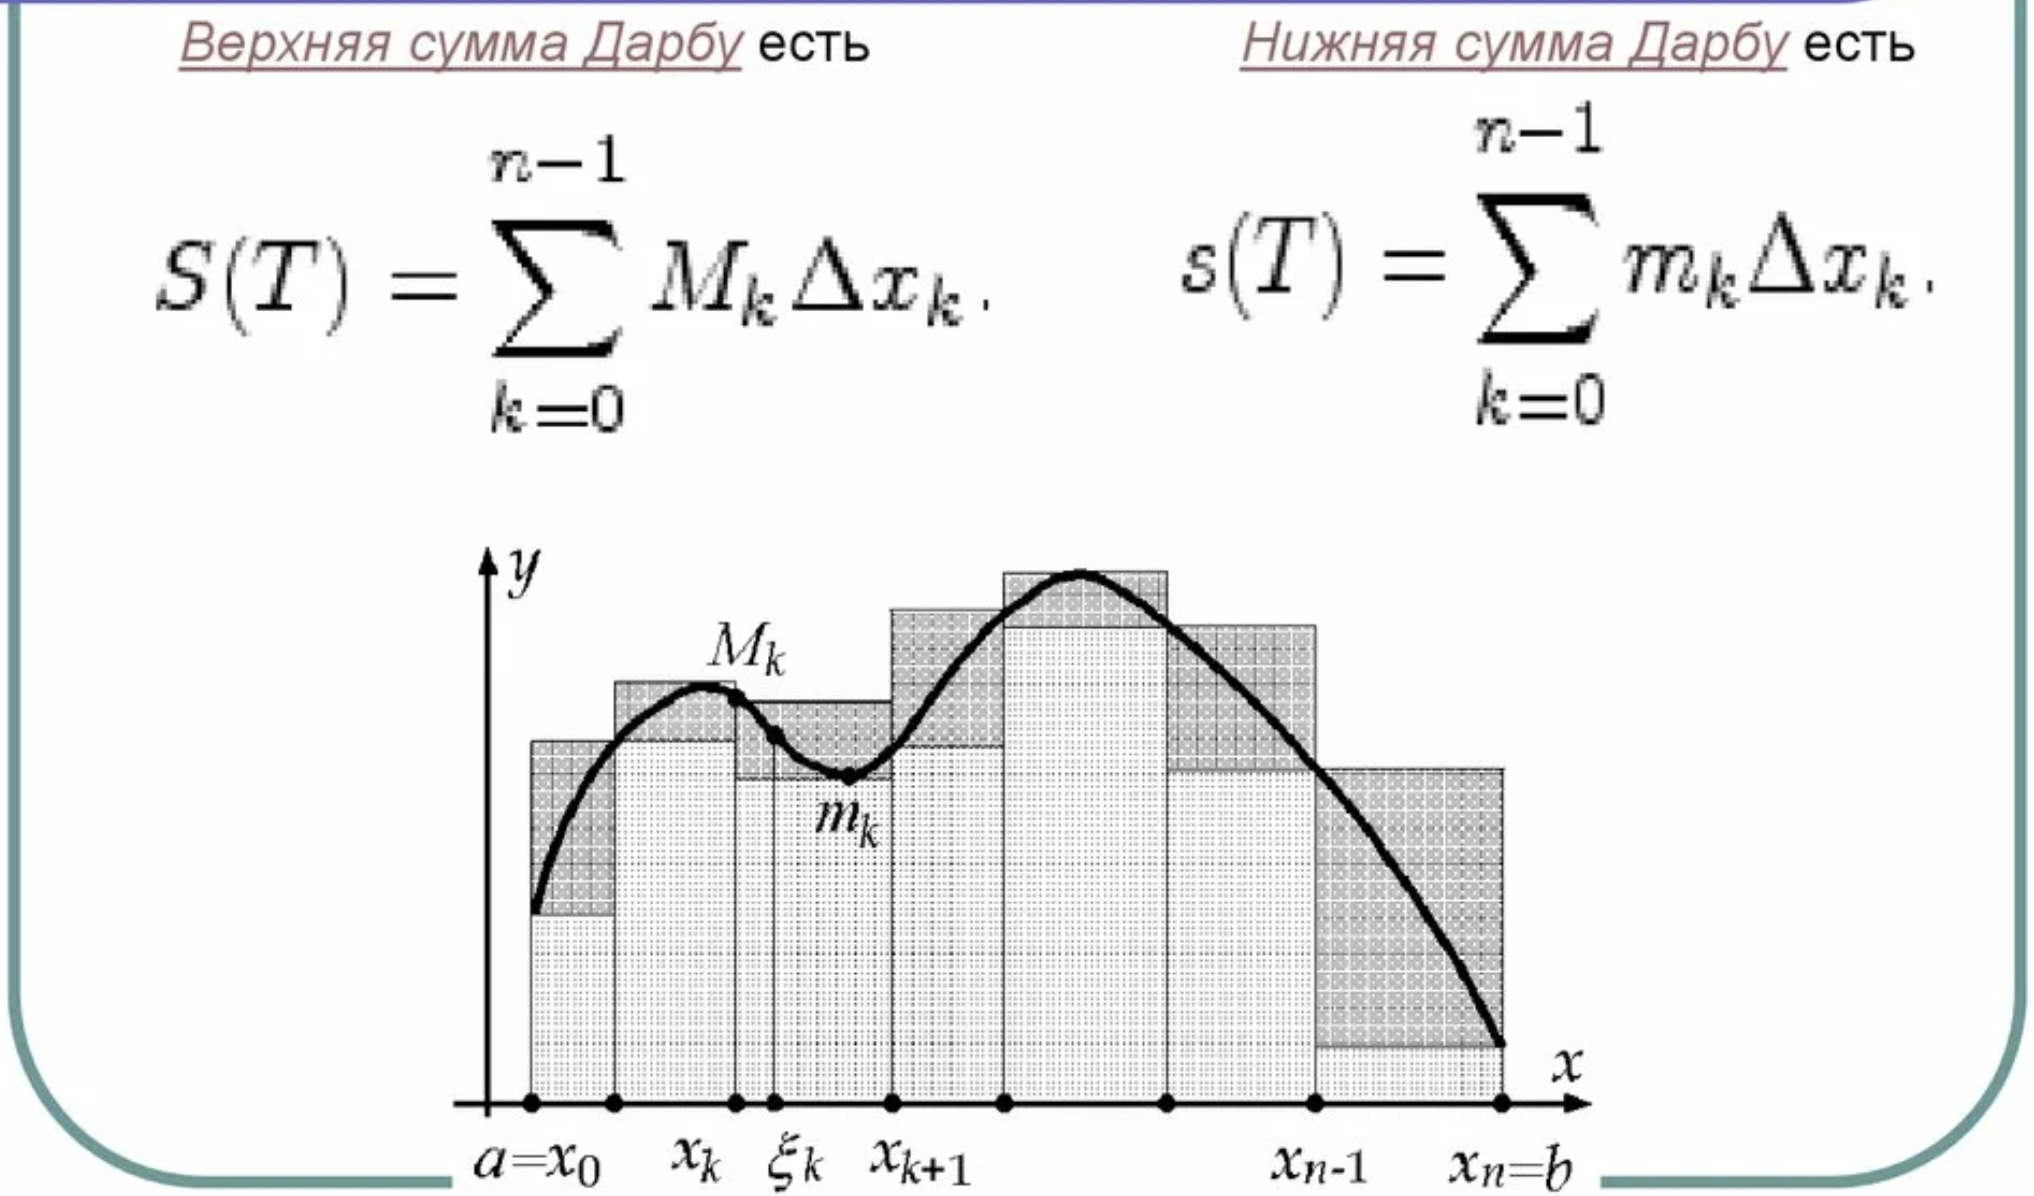
\includegraphics[width=0.42\textwidth]{darbu.png}
    \nopagebreak
    \\ \vspace{0.3em} \small\itshape Рис. 11.1: А вот и они
\end{center}

\begin{itemize}
    \item \textbf{Монотонность:} Добавление точки делит один столбик на два узких. Локальные минимумы на половинках могут стать только выше общего старого минимума. «Пол» приподнимается (площадь растет). Локальные максимумы — только ниже, «потолок» проседает (площадь падает).
    \item \textbf{Смысл оценки $p(M-m)\lambda(T)$:} При добавлении одной точки изменение площади происходит только внутри одного исходного отрезка. Его ширина не превышает $\lambda(T)$, а максимальный перепад высоты функции от самого дна до пика равен $(M-m)$. Значит, от одной точки мы выигрываем/теряем максимум площадь одного такого прямоугольника: $(M-m)\lambda(T)$. Если точек $p$ штук, то суммарный эффект не превысит $p(M-m)\lambda(T)$.
\end{itemize}

\paragraph{Доказательство в 4 коротких шага.}

\begin{enumerate}
    \item \textbf{Выделение изменяемого участка ($p=1$):}
    Пусть в разбиение $T$ добавлена одна точка $x^*$, попавшая внутрь отрезка $[x_{k-1}, x_k]$. Обозначим инфимумы на двух новых половинках как $m'_1$ и $m'_2$. Поскольку точная нижняя грань на подмножестве не может быть меньше грани на всем множестве, имеем: $m'_1 \ge m_k$ и $m'_2 \ge m_k$.
    
    Разность новых и старых нижних сумм возникает исключительно на этом отрезке:
    $$ s(f, T') - s(f, T) = m'_1 (x^* - x_{k-1}) + m'_2 (x_k - x^*) - m_k \Delta x_k $$

    \item \textbf{Алгебраический трюк с точкой $x^*$:}
    Распишем длину старого отрезка через тождественное добавление и вычитание точки $x^*$: $\Delta x_k = x_k - x_{k-1} = (x^* - x_{k-1}) + (x_k - x^*)$. Подставим это в формулу разности и сгруппируем члены при одинаковых скобках длины:
    $$ s(f, T') - s(f, T) = \underbrace{(m'_1 - m_k)}_{\ge 0} \underbrace{(x^* - x_{k-1})}_{> 0} + \underbrace{(m'_2 - m_k)}_{\ge 0} \underbrace{(x_k - x^*)}_{> 0} \ge 0 \implies s(f, T) \le s(f, T') $$
    Для верхних сумм аналогично через супремумы ($M'_1 \le M_k, M'_2 \le M_k$):
    $$ S(f, T) - S(f, T') = \underbrace{(M_k - M'_1)}_{\ge 0} (x^* - x_{k-1}) + \underbrace{(M_k - M'_2)}_{\ge 0} (x_k - x^*) \ge 0 \implies S(f, T') \le S(f, T) $$

    \item \textbf{Вывод оценки для одной точки:}
    Оценим сверху разность нижних сумм из предыдущего шага. Так как $m'_1 \le M$ (глобальный супремум), а $m_k \ge m$ (глобальный инфимум), то каждая разность инфимумов не превышает полный размах функции: $(m'_1 - m_k) \le M - m$ и $(m'_2 - m_k) \le M - m$. Вынесем $(M-m)$ за скобки:
    $$ s(f, T') - s(f, T) \le (M - m) \big[ (x^* - x_{k-1}) + (x_k - x^*) \big] = (M - m)\Delta x_k $$
    Учитывая, что длина любого отрезка не больше мелкости разбиения ($\Delta x_k \le \lambda(T)$), получаем:
    $$ s(f, T') - s(f, T) \le (M - m)\lambda(T) $$

    \item \textbf{Переход к произвольному числу $p$ точек:}
    Если добавляется $p$ точек, будем вводить их поочередно, выстраивая цепочку разбиений: $T = T_0 \subset T_1 \subset \dots \subset T_p = T'$. При каждом добавлении одной точки мелкость текущего разбиения не превосходит исходную: $\lambda(T_i) \le \lambda(T)$.
    Складывая $p$ полученных на каждом шаге одинаковых оценок, по правилу телескопической суммы имеем:
    $$ s(f, T') - s(f, T) = \sum_{i=1}^p \big(s(f, T_i) - s(f, T_{i-1})\big) \le \sum_{i=1}^p (M - m)\lambda(T) = p(M - m)\lambda(T) $$
    Доказательство для верхних сумм проводится зеркально. Лемма полностью доказана.
\end{enumerate}


% --- Вопрос 12 ---
\examquestion{12}{Критерий интегрируемости в терминах сумм Дарбу}
{Сформулируйте и проведите доказательство теоремы: Критерий интегрируемости Дарбу. Проработайте доказательство в обе стороны (необходимость и достаточность).}

\paragraph{Базовые понятия и обозначения.}
Для любого разбиения $T$ отрезка $[a, b]$ определены нижняя $s(f, T)$ и верхняя $S(f, T)$ суммы Дарбу.
\begin{itemize}
    \item \textbf{Интегралы Дарбу:} Нижним интегралом Дарбу $I_*$ называется супремум всех нижних сумм, а верхним интегралом $I^*$ — инфимум всех верхних сумм по всем возможным разбиениям:
    $$ I_* = \sup_{T} s(f, T), \quad I^* = \inf_{T} S(f, T) $$
    \item \textbf{Интегрируемость по Риману:} Ограниченная функция $f(x)$ называется интегрируемой по Риману ($f \in \mathcal{R}[a,b]$), если её верхний и нижний интегралы Дарбу совпадают. Их общее значение равно интегралу Римана: $I_* = I^* = I$.
    \item \textbf{Смысл оценки:} Разность $S(f, T) - s(f, T)$ — это суммарная площадь «зазоров» между накрывающей и вписанной ступенчатыми фигурами. Функция интегрируема тогда и только тогда, когда этот зазор можно сжать до сколь угодно малой величины $\varepsilon$.
\end{itemize}

\paragraph{Формулировка теоремы (Критерий Дарбу).}
Ограниченная на отрезке $[a, b]$ функция $f(x)$ интегрируема по Риману на этом отрезке тогда и только тогда, когда для любого $\varepsilon > 0$ существует такое разбиение $T$, при котором:
\begin{tcolorbox}[colback=white, colframe=black, boxrule=0.5pt, arc=0pt, borderline={0.5pt}{0pt}{black, dashed}]
$$ f \in \mathcal{R}[a,b] \iff \forall \varepsilon > 0 \;\; \exists T : \;\; S(f, T) - s(f, T) < \varepsilon $$
\end{tcolorbox}

\paragraph{Доказательство необходимости ($\implies$).}
Пусть функция интегрируема, то есть $I_* = I^* = I$. Зафиксируем произвольное $\varepsilon > 0$.
\begin{enumerate}
    \item По определению супремума, для величины $\frac{\varepsilon}{2}$ найдется разбиение $T_1$, нижняя сумма которого близка к $I$:
    $$ s(f, T_1) > I - \frac{\varepsilon}{2} $$
    \item По определению инфимума, для величины $\frac{\varepsilon}{2}$ найдется разбиение $T_2$, верхняя сумма которого близка к $I$:
    $$ S(f, T_2) < I + \frac{\varepsilon}{2} $$
    \item Построим общее измельчение $T = T_1 \cup T_2$. По лемме об изменении сумм, при добавлении новых точек нижняя сумма может только вырасти, а верхняя — только уменьшиться. Тогда справедливы два раздельных неравенства:
    $$ s(f, T) \ge s(f, T_1) > I - \frac{\varepsilon}{2} \implies -s(f, T) < -I + \frac{\varepsilon}{2} $$
    $$ S(f, T) \le S(f, T_2) < I + \frac{\varepsilon}{2} $$
    Сложим эти два неравенства для одного и того же разбиения $T$:
    $$ S(f, T) - s(f, T) < \left(I + \frac{\varepsilon}{2}\right) + \left(-I + \frac{\varepsilon}{2}\right) = \varepsilon $$
\end{enumerate}
Необходимость доказана.

\paragraph{Доказательство достаточности ($\impliedby$).}
Пусть условие выполнено: для любого $\varepsilon > 0$ существует разбиение $T$, при котором $S(f, T) - s(f, T) < \varepsilon$.

По определению интегралов Дарбу как точных граней, для абсолютно любого разбиения $T$ выполнены стандартные ограничения: $s(f, T) \le I_*$ и $I^* \le S(f, T)$. Избавимся от тройного неравенства и запишем это в виде двух простых утверждений:
\begin{enumerate}
    \item Так как $I^* \le S(f, T)$ и $-I_* \le -s(f, T)$, мы можем оценить разность интегралов сверху через разность сумм на данном разбиении:
    $$ I^* - I_* \le S(f, T) - s(f, T) $$
    \item Поскольку по условию эта разность сумм меньше $\varepsilon$, получаем:
    $$ 0 \le I^* - I_* < \varepsilon $$
\end{enumerate}
Постоянная величина $I^* - I_*$ неотрицательна и при этом строго меньше любого сколь угодно малого положительного числа $\varepsilon$. Это возможно только если эта разность равна нулю:
$$ I^* - I_* = 0 \implies I_* = I^* $$
По определению это означает, что функция интегрируема по Риману. Достаточность доказана.

% --- Вопрос 13 ---
\examquestion{13}{Интегрируемость непрерывных функций}
{Сформулируйте и докажите теорему об интегрируемости по Риману любой функции, непрерывной на сегменте $[a, b]$ ($C[a,b]\subset\mathcal{R}[a,b]$). Покажите, на каком именно этапе доказательства и для чего необходимо применять теорему Кантора о равномерной непрерывности.}

\paragraph{Используемые теоремы.}
Для доказательства опираемся на три факта:
\begin{itemize}
    \item \textbf{Вторая теорема Вейерштрасса:} Непрерывная на отрезке функция всегда достигает на нем своих точных граней (максимума и минимума).
    \item \textbf{Теорема Кантора:} Непрерывная на замкнутом отрезке функция равномерно непрерывна. То есть для любого $\varepsilon > 0$ существует единое $\delta > 0$, такое что при $|x' - x''| < \delta$ всегда выполняется $|f(x') - f(x'')| < \varepsilon$.
    \item \textbf{Критерий Дарбу:} Функция интегрируема, если $\forall \varepsilon > 0 \exists T: S(f, T) - s(f, T) < \varepsilon$.
\end{itemize}

\paragraph{Формулировка теоремы.}
Если функция $f(x)$ непрерывна на сегменте $[a, b]$, то она интегрируема по Риману на этом сегменте.

\paragraph{Тезисное доказательство.}
\begin{enumerate}
    \item Зададим произвольное $\varepsilon > 0$. 
    \item \textbf{Применяем теорему Кантора:} Для величины $\frac{\varepsilon}{b-a} > 0$ существует \textit{общее} $\delta > 0$, такое что для любых точек, расстояние между которыми меньше $\delta$, разность значений функции строго меньше $\frac{\varepsilon}{b-a}$.
    \item Возьмем любое разбиение $T$ с мелкостью $\lambda(T) < \delta$. Это значит, что длина каждого $k$-го отрезка $\Delta x_k < \delta$.
    \item На каждом отрезке $[x_{k-1}, x_k]$ функция непрерывна. По \textbf{теореме Вейерштрасса} она достигает внутри него инфимума $m_k$ и супремума $M_k$ в конкретных точках $x'_k$ и $x''_k$.
    \item Так как обе эти точки лежат внутри одного отрезка, расстояние между ними меньше $\delta$. Значит, размах функции на этом участке ограничен:
    $$ M_k - m_k < \frac{\varepsilon}{b-a} $$
    \item Составим разность сумм Дарбу для всего разбиения и заменим скобки с размахом на нашу оценку:
    $$ S(f, T) - s(f, T) = \sum_{k=1}^n (M_k - m_k)\Delta x_k < \sum_{k=1}^n \frac{\varepsilon}{b-a}\Delta x_k $$
    \item Выносим константу за сумму. Сумма длин всех подотрезков равна $(b-a)$:
    $$ \frac{\varepsilon}{b-a} \sum_{k=1}^n \Delta x_k = \frac{\varepsilon}{b-a}(b-a) = \varepsilon $$
    \item Получили $S(f, T) - s(f, T) < \varepsilon$. По критерию Дарбу функция интегрируема.
\end{enumerate}

\paragraph{Интуитивный смысл («на пальцах»).}
Обычная непрерывность гарантирует, что график плавный, но масштаб этой плавности (своё $\delta$) в каждой точке может быть разным. Теорема Кантора спасает ситуацию: она разрешает выбрать \textbf{одно общее, самое строгое $\delta$} для всего отрезка. Если нарезать ось $x$ на кусочки мельче этого $\delta$, колебания графика внутри \textit{каждой} ячейки одновременно станут микроскопическими. Суммарная площадь "зазоров" между ступенчатыми фигурами Дарбу схлопнется до нуля, и интеграл возьмется.



% --- Вопрос 14 ---
\examquestion{14}{Интегрируемость монотонных функций}
{Сформулируйте и докажите теорему об интегрируемости монотонной функции на сегменте $[a, b]$. Проведите доказательство через телескопическую оценку разности сумм Дарбу. Проведите сравнительный анализ: почему для монотонных функций не нужна теорема Кантора?}

\paragraph{Формулировка теоремы.}
Если функция $f(x)$ монотонна на сегменте $[a, b]$, то она интегрируема на этом сегменте.

\paragraph{Доказательство.}
Пусть $f(x)$ монотонно не убывает. Если $f(a) = f(b)$, функция константна и интегрируема. Рассмотрим случай $f(b) > f(a)$.

Зададим $\varepsilon > 0$. Разделим $[a, b]$ на $n$ равных частей длиной $\Delta x = \frac{b-a}{n}$. 
Из-за монотонности точные грани на каждом отрезке $[x_{k-1}, x_k]$ достигаются на его концах:
$$ m_k = f(x_{k-1}), \quad M_k = f(x_k) $$

Разность сумм Дарбу принимает вид:
$$ S(f, T) - s(f, T) = \sum_{k=1}^n (M_k - m_k) \Delta x = \frac{b-a}{n} \sum_{k=1}^n (f(x_k) - f(x_{k-1})) $$

Сумма внутри — телескопическая: все промежуточные значения $f(x_k)$ сокращаются, остаются только края:
$$ \sum_{k=1}^n (f(x_k) - f(x_{k-1})) = f(x_n) - f(x_0) = f(b) - f(a) $$

Итоговая разность:
$$ S(f, T) - s(f, T) = \frac{b-a}{n} (f(b) - f(a)) $$

Для любого заданного $\varepsilon$ мы можем выбрать столь большое количество разбиений $n$, чтобы это выражение стало меньше $\varepsilon$. Так как при любом $n$ мы можем подобрать такое разбиение, условие критерия Дарбу выполняется. Интегрируемость доказана.

\paragraph{Почему не нужна теорема Кантора?}
Для непрерывных функций мы не знаем, где внутри отрезка лежат экстремумы, поэтому вынуждены принудительно ограничивать колебания через равномерную непрерывность (теорему Кантора). 
У монотонной функции экстремумы всегда «сидят» на концах отрезков. Из-за этого суммарная ошибка разбиения зависит только от разности значений в крайних точках всего сегмента $[a, b]$, а не от «поведения» функции внутри. Монотонность сама по себе жестко ограничивает накопленную погрешность: сколько бы разрывов ни было внутри, они все «схлопываются» при телескопическом сокращении.

% --- Вопрос 15 ---
\examquestion{15}{Интегрируемость функций с конечным числом разрывов}
{Сформулируйте и докажите теорему об интегрируемости ограниченной функции, имеющей конечное число точек разрыва на сегменте $[a, b]$. Примените метод «изоляции». Обоснуйте важность ограниченности функции (пример $1/x$).}

\paragraph{Формулировка теоремы.}
Если функция $f(x)$ ограничена на сегменте $[a, b]$ и имеет на нем конечное число точек разрыва, то она интегрируема на этом сегменте.

\paragraph{Доказательство (Метод «изоляции»).}
Пусть функция ограничена: существует такое число $M>0$, что $-M \le f(x) \le M$ для всех $x \in [a,b]$ (функция зажата в коридоре высотой $2M$). 

Проведем доказательство для одной точки разрыва $c \in (a, b)$ (для $k$ точек алгоритм аналогичен). Зададим произвольное $\varepsilon > 0$.

\begin{enumerate}
    \item \textbf{Шаг 1. Изолируем разрыв.} Окружим точку $c$ интервалом $(c - \delta, c + \delta)$. Длина этого центрального отрезка разбиения равна $\Delta x_c = (c + \delta) - (c - \delta) = 2\delta$.
    \item \textbf{Шаг 2. Выбираем ширину.} Мы сами вправе выбрать $\delta$ сколь угодно малым. Сожмем его так, чтобы выполнялось условие: $4M\delta < \frac{\varepsilon}{2}$.
    \item \textbf{Шаг 3. Работаем с остатком.} Вне этого интервала остаются два чистых сегмента: $[a, c - \delta]$ и $[c + \delta, b]$. На них функция непрерывна, а значит, интегрируема. По критерию Дарбу для них найдутся такие разбиения $T_1$ и $T_2$, что разности их сумм ничтожно малы:
    $$ S(T_1) - s(T_1) < \frac{\varepsilon}{4} \quad \text{и} \quad S(T_2) - s(T_2) < \frac{\varepsilon}{4} $$
\end{enumerate}

Объединим разбиения $T_1, T_2$ и центральный отрезок $[c - \delta, c + \delta]$ в единое полное разбиение $T$ всего сегмента $[a, b]$. Полная разность сумм Дарбу распадается на три части:
$$ S(f, T) - s(f, T) = \underbrace{\big(S(T_1) - s(T_1)\big)}_{< \varepsilon/4} + \underbrace{(M_c - m_c)\Delta x_c}_{\text{окрестность } c} + \underbrace{\big(S(T_2) - s(T_2)\big)}_{< \varepsilon/4} $$

\paragraph{Подробная оценка центрального слагаемого:}
\begin{itemize}
    \item Так как функция зажата в пределах от $-M$ до $+M$, её максимальное значение $M_c \le M$, а минимальное $m_c \ge -M$. 
    \item Значит, максимальный размах (колебание) функции на отрезке не может превысить: $(M_c - m_c) \le M - (-M) = 2M$.
    \item Длина отрезка равна $\Delta x_c = 2\delta$.
    \item Перемножаем их: $(M_c - m_c)\Delta x_c \le 2M \cdot 2\delta = 4M\delta$.
    \item А так как на Шаге 2 мы сами зафиксировали, что $4M\delta < \frac{\varepsilon}{2}$, то центральное слагаемое железно меньше $\frac{\varepsilon}{2}$.
\end{itemize}

Собираем все три части суммы вместе:
$$ S(f, T) - s(f, T) < \frac{\varepsilon}{4} + \frac{\varepsilon}{2} + \frac{\varepsilon}{4} = \varepsilon $$
Разность сумм Дарбу оказалась меньше $\varepsilon$. По критерию Дарбу функция интегрируема.

\vspace{0.5em}
\begin{center}
\begin{tikzpicture}[scale=0.9, every node/.style={scale=0.9}]
    \draw[->, thick] (0,0) -- (6,0) node[right] {$x$};
    \draw[->, thick] (0,0) -- (0,3) node[above] {$y$};
    
    % График функции с разрывом
    \draw[thick, blue] (0.5, 2) .. controls (1.5, 2) .. (2.5, 1);
    \draw[thick, blue] (3.5, 2.5) .. controls (4.5, 2.5) .. (5.5, 1.5);
    \filldraw[blue] (2.5, 1) circle (2pt);
    \draw[blue, fill=white, thick] (3.5, 2.5) circle (2pt);
    
    % Изолирующий пакет
    \draw[dashed, red, fill=red!10, thick] (2.5,0) rectangle (3.5, 2.6);
    \node[red, align=center] at (3, 3) {Изолирующий \\ пакет $\Delta x_c$};
    
    % Подписи
    \draw[thick] (2.5, 0.1) -- (2.5, -0.1) node[below] {$c-\delta$};
    \draw[thick] (3.5, 0.1) -- (3.5, -0.1) node[below] {$c+\delta$};
    \node[below=10pt, red] at (3, 0) {$c$};
\end{tikzpicture}
\end{center}
\vspace{0.5em}

\paragraph{Важность условия ограниченности (Пример $1/x$).}
Метод изоляции работает **только** если высота изолирующего прямоугольника ограничена константой $M$. Если функция улетает в бесконечность, метод ломается.
Рассмотрим функцию $f(x) = \frac{1}{x}$ на интервале $(0, 1)$, доопределив её в нулю ($f(0) = 0$). У неё одна точка разрыва ($x = 0$).

Для любого разбиения $T$ самый первый отрезок $[0, x_1]$ содержит разрыв. Точная верхняя грань функции на нём бесконечна: $M_1 = \sup_{[0, x_1]} \frac{1}{x} = +\infty$.
Из-за этого верхняя сумма Дарбу всегда «взрывается»:
$$ S(f, T) = \underbrace{M_1 \cdot \Delta x_1}_{+\infty} + \sum_{k=2}^n M_k \Delta x_k = +\infty $$
Разность $S(f,T) - s(f,T) = +\infty$. Критерий Дарбу не выполняется, интеграл Римана не существует.

\vspace{0.5em}
\begin{center}
\begin{tikzpicture}[scale=0.9, every node/.style={scale=0.9}]
    \draw[->, thick] (0,0) -- (5,0) node[right] {$x$};
    \draw[->, thick] (0,0) -- (0,4) node[above] {$y$};
    
    % График 1/x
    \draw[domain=0.25:4.5, smooth, variable=\x, thick, blue] plot ({\x}, {1/\x});
    
    % Бесконечный прямоугольник
    \draw[fill=red!20, thick] (0, 0) rectangle (1.2, 3.8);
    \draw[->, thick, red] (0.6, 2.5) -- (0.6, 4.2) node[above] {$M_1 \to +\infty$};
    \node[red, align=center] at (2.5, 3.0) {Площадь первого \\ пакета $\to \infty$};
    
    % Подписи
    \draw[thick] (1.2, 0.1) -- (1.2, -0.1) node[below] {$x_1$};
\end{tikzpicture}
\end{center}
\vspace{0.5em}

\end{document}